%%%%%%%%%%%%%%%%%%%%%%%%%%%%%%%%%%%%%%%%%
% Wenneker Assignment
% LaTeX Template
% Version 2.0 (12/1/2019)
%
% This template originates from:
% http://www.LaTeXTemplates.com
%
% Authors:
% Vel (vel@LaTeXTemplates.com)
% Frits Wenneker
%
% License:
% CC BY-NC-SA 3.0 (http://creativecommons.org/licenses/by-nc-sa/3.0/)
% 
%%%%%%%%%%%%%%%%%%%%%%%%%%%%%%%%%%%%%%%%%

%----------------------------------------------------------------------------------------
%	PACKAGES AND OTHER DOCUMENT CONFIGURATIONS
%----------------------------------------------------------------------------------------

\documentclass[11pt]{scrartcl} % Font size

%%%%%%%%%%%%%%%%%%%%%%%%%%%%%%%%%%%%%%%%%
% Wenneker Assignment
% Structure Specification File
% Version 2.0 (12/1/2019)
%
% This template originates from:
% http://www.LaTeXTemplates.com
%
% Authors:
% Vel (vel@LaTeXTemplates.com)
% Frits Wenneker
%
% License:
% CC BY-NC-SA 3.0 (http://creativecommons.org/licenses/by-nc-sa/3.0/)
% 
%%%%%%%%%%%%%%%%%%%%%%%%%%%%%%%%%%%%%%%%%

%----------------------------------------------------------------------------------------
%	PACKAGES AND OTHER DOCUMENT CONFIGURATIONS
%----------------------------------------------------------------------------------------

\usepackage{amsmath, amsfonts, amsthm} % Math packages

\usepackage{listings} % Code listings, with syntax highlighting

\usepackage[english]{babel} % English language hyphenation

\usepackage{graphicx} % Required for inserting images
\usepackage{caption}
\graphicspath{{Figures/}{./}} % Specifies where to look for included images (trailing slash required)

\usepackage{booktabs} % Required for better horizontal rules in tables

\numberwithin{equation}{section} % Number equations within sections (i.e. 1.1, 1.2, 2.1, 2.2 instead of 1, 2, 3, 4)
\numberwithin{figure}{section} % Number figures within sections (i.e. 1.1, 1.2, 2.1, 2.2 instead of 1, 2, 3, 4)
\numberwithin{table}{section} % Number tables within sections (i.e. 1.1, 1.2, 2.1, 2.2 instead of 1, 2, 3, 4)

\setlength\parindent{0pt} % Removes all indentation from paragraphs

\usepackage{enumitem} % Required for list customisation
\setlist{noitemsep} % No spacing between list items

%----------------------------------------------------------------------------------------
%	DOCUMENT MARGINS
%----------------------------------------------------------------------------------------

\usepackage{geometry} % Required for adjusting page dimensions and margins

\geometry{
	paper=a4paper, % Paper size, change to letterpaper for US letter size
	top=2.5cm, % Top margin
	bottom=3cm, % Bottom margin
	left=3cm, % Left margin
	right=3cm, % Right margin
	headheight=0.75cm, % Header height
	footskip=1.5cm, % Space from the bottom margin to the baseline of the footer
	headsep=0.75cm, % Space from the top margin to the baseline of the header
	%showframe, % Uncomment to show how the type block is set on the page
}

%----------------------------------------------------------------------------------------
%	FONTS
%----------------------------------------------------------------------------------------

\usepackage[utf8]{inputenc} % Required for inputting international characters
\usepackage[T1]{fontenc} % Use 8-bit encoding

\usepackage{fourier} % Use the Adobe Utopia font for the document

%\usepackage[framed,numbered,autolinebreaks,useliterate]{mcode}

%----------------------------------------------------------------------------------------
%	SECTION TITLES
%----------------------------------------------------------------------------------------

\usepackage{sectsty} % Allows customising section commands

\sectionfont{\normalfont\bfseries} % \section{} styling
\subsectionfont{\normalfont\bfseries} % \subsection{} styling
\subsubsectionfont{\normalfont\itshape} % \subsubsection{} styling
\paragraphfont{\normalfont\scshape} % \paragraph{} styling

%----------------------------------------------------------------------------------------
%	HEADERS AND FOOTERS
%----------------------------------------------------------------------------------------

\usepackage{scrlayer-scrpage} % Required for customising headers and footers

\ohead*{} % Right header
\ihead*{} % Left header
\chead*{} % Centre header

\ofoot*{} % Right footer
\ifoot*{} % Left footer
\cfoot*{\pagemark} % Centre footer

% MY PACKAGES
%\usepackage[framed,numbered,autolinebreaks,useliterate]{mcode}
\usepackage{listings}
\usepackage{float}
\usepackage{amsmath}
\usepackage{tikz}
\usetikzlibrary{shapes,arrows,positioning}
\usepackage{hyperref} % Include the file specifying the document structure and custom commands

%----------------------------------------------------------------------------------------
%	TITLE SECTION
%----------------------------------------------------------------------------------------

\title{	
	\normalfont\normalsize
	\textsc{Universität Würzburg}\\ % Your university, school and/or department name(s)
	\vspace{25pt} % Whitespace
	\rule{\linewidth}{0.5pt}\\ % Thin top horizontal rule
	\vspace{20pt} % Whitespace
	{\huge Übung 2: Übertragungsfunktion, Regelkreis}\\ % The assignment title
	\vspace{12pt} % Whitespace
	\rule{\linewidth}{2pt}\\ % Thick bottom horizontal rule
	\vspace{12pt} % Whitespace
}

\author{\LARGE Alexander Björk, Janis Kaltenthaler} % Your name

\date{\normalsize\today} % Today's date (\today) or a custom date

\begin{document}

\maketitle % Print the title

%----------------------------------------------------------------------------------------
%	FIGURE EXAMPLE
%----------------------------------------------------------------------------------------

\section*{Aufgabe 2-1. Übertragungsfunktion des PT$_2$-Gliedes (4 Punkte)}
\subsection*{a) $d>1$}
\textbf{Pole:}\\
\begin{equation*}
s_{1/2}=-d\omega_0\pm\omega_0\sqrt{d^2-1}
\end{equation*}
Die Terme, der bereits angegebenen Pole lassen sich nicht weiter vereinfachen. Es lässt sich jedoch zeigen, dass die Realteile (also $s_1$ und $s_2$, weil der Imaginärteil durch $d>1$ Null wird) für beide negativ sind.
Durch $d^2-1<1$ gilt auch
\begin{equation*}
s_{1/2}=\omega_0 \left( -d \pm \sqrt{d^2-1} \right) < 0.
\end{equation*}
Damit klingt das Übergangsverhalten für $t \rightarrow \infty$ ab und am Ausgang ist nur noch das stationäre Verhalten zu beobachten. \\

\textbf{Sprungantwort im Frequenzbereich:}\\
Die Sprungantwort im Frequenzbereich erhält man indem man die Übertragungsfunktion nach $Y(s)$ umstellt und den Laplace-transformierten Einheitssprung als Eingabe $U(s)$ verwendet. Der Einheitssprung $\sigma(t)$ ist definiert als
\begin{equation*}
\sigma(t)=\int_{0}^tc^Ta^{At}bd\tau + d.
\end{equation*}
Als Laplace-transformierte Eingabe $U(s)$ heißt das
\begin{equation*}
U(s) = \dfrac{1}{s}.
\end{equation*}
Durch Einsetzen in die Übertragungsfunktion und anschließendem Umstellen erhält man
\begin{equation*}
Y(s)=\dfrac{k}{\dfrac{1}{{\omega_0}^2}s^3+\dfrac{2d}{\omega_0}s^2+s}
\end{equation*}
als Sprungantwort im Frequenzbereich. \\

\textbf{Sprungantwort im Zeitbereich:}\\
Die Sprungantwort im Zeitbereich erhält man durch die Laplace-Transformation der Sprungantwort im Frequenzbereich. Durch Substitution von von $T:=\dfrac{1}{\omega_0}$ erhält man die etwas vereinfachte Übertragungsfunktion
\begin{equation*}
Y(s)=\dfrac{k}{T^2s^3+2dTs^2+s}.
\end{equation*}
Damit erhält man im Zeitbereich eine Sprungantwort von
\begin{equation*}
y(t) = k \left(1-\dfrac{E_1\left(\sqrt{d^2-1}+d\right) + E_2\left(\sqrt{d^2-1}-d\right)}{2 \sqrt{d^2-1}}\right)
\end{equation*}
mit
\begin{equation*}
E_{1,2} = \text{exp}\left(\dfrac{t}{T}\left(\pm\sqrt{d^2-1}-d\right)\right).
\end{equation*}\\

\textbf{Zeitlicher Verlauf von $y(t)$:}\\
Die Funktion nähert sich mit einem klassischen Verlauf einer $k \cdot exp\left(-\dfrac{1}{t}\right)$ Kurve dem Grenzwert $k$ an.

\subsection*{b) $d=1$}
\textbf{Pole:}\\
Für den Fall $d=1$ gibt es nur noch einen Pol mit
\begin{equation*}
s_1 = s_2 = s = -\omega_0.
\end{equation*}
Dadurch vereinfacht sich die Übertragunsfunktion mit $T:=\dfrac{1}{\omega_0}$ zu
\begin{equation*}
G(s) = \dfrac{k}{T^2s^2+2Ts+1}.
\end{equation*} \\

\textbf{Sprungantwort im Frequenzbereich:}\\
Die Sprungantwort im Frequenzbereich ist
\begin{equation*}
Y(s)=\dfrac{k}{T^2s^3+2Ts^2+s}.
\end{equation*} \\

\textbf{Sprungantwort im Zeitbereich:}\\
Die Sprungantwort im Zeitbereich ist
\begin{equation*}
y(t)=k \left( 1-\text{exp}\left( -\dfrac{t}{T} \right) - \dfrac{\text{exp}\left( -\dfrac{t}{T} \right)t}{T} \right).
\end{equation*}\\

\textbf{Zeitlicher Verlauf von $y(t)$:}\\
Der zeitliche Verlauf von $y(t)$ für $d=1$ ist qualitativ der selbe wie für $d>1$. Auch hier stellt sich ein stationäres Verhalten bei $k$ ein.


\subsection*{c) $d=0$}
\textbf{Pole:}\\
Durch $d=0$ sind die Pole nun komplex mit $\Re(s)=0$.
\begin{equation*}
s_{1/2}=\pm \omega_0 i
\end{equation*}
Diesen Polstellen weisen auf ein oszillierendes System hin.\\

\textbf{Sprungantwort im Frequenzbereich:}\\
\begin{equation*}
Y(s)=\dfrac{k}{T^2s^3+s}
\end{equation*}\\

\textbf{Sprungantwort im Zeitbereich:}\\
Die Sprungantwort im Zeitbereich bestätigt die Aussage über die Polstellen:
\begin{equation*}
y(t)=k \left( 1 - \cos \left( \dfrac{t}{T} \right) \right)
\end{equation*}
Wir haben ein osziliierendes System mit Amplitude $k$ und Schwingungsdauer $\tilde{T}=2\pi n T$ für $n \in \mathbb{Z}$.\\

\textbf{Zeitlicher Verlauf von $y(t)$:}\\
Es stellt sich durch das oszillierende Verhalten kein stationärer Zustand ein. Der zeitliche Verlauf entspricht dem einer klassischen Cosinus-Kurve.


\subsection*{d) $0<d<1$}
\textbf{Pole:}\\
Die Pole lassen sich hier nicht vereinfachen. Es ist jedoch möglich sie nun sinnvoll in Real- und Imaginärteil anzugeben, da nun beide verschieden von Null sind.
\begin{align*}
s_{1/2}&=-d\omega_0\pm\omega_0\sqrt{d^2-1} \\
\Re(s_{1/2})&=-d\omega_0 \\
\Im(s_{1/2})&=\pm\omega_0\sqrt{d^2-1}
\end{align*}
Der negative Realteil zeigt an, dass hier entweder ein stabiles oder ein abklingendes System vorliegt. Der von Null verschiedene Imaginärteil zeigt an, dass es sich um ein oszillierendes System handelm muss.\\

\textbf{Sprungantwort im Frequenzbereich:}\\
Die Sprungantwort im Frequenzbereich lässt sich nicht vereinfachen.
\begin{equation*}
Y(s)=\dfrac{k}{T^2s^3+2dTs^2+s}.
\end{equation*}\\

\textbf{Sprungantwort im Zeitbereich:}\\
Die Sprungantwort im Zeitbereich ist die selbe wie für $d>1$.
\begin{equation*}
y(t) = k \left(1-\dfrac{E_1\left(\sqrt{d^2-1}+d\right) + E_2\left(\sqrt{d^2-1}-d\right)}{2 \sqrt{d^2-1}}\right)
\end{equation*}\\

\textbf{Zeitlicher Verlauf von $y(t)$:}\\
Wie eingangs beschrieben liegt hier ein oszillierendes System vor, welches mit der Zeit abklingt (gedämpfte Cosinus-Schwingung) während es um $k$ schwingt. Mit der Zeit stellt sich ein stationäres Verhalten um $k$ ein.



\section*{Aufgabe 2-2. Übertragungsfunktion im Regelkreis (6 Punkte)}
\subsection*{a)}
Es gelten folgende Zusammenhänge:
\begin{align*}
Y(s)&=G(s)U(s) \\
\hat{Y}(s)&=\tilde{Y}(s)+R(s)\\
U(s)&=E(s)K(s)\\
E(s)&=W(s)-\hat{Y}(s)\\
\tilde{Y}(s)&=Y(s)C(s)
\end{align*}

\subsection*{b)}
Die Führungsübertragungsfuntion berechnet sich mit $G_w(s)=\dfrac{Y(s)}{W(s)}$ mit $R(s)=0$. Für die Regelgröße ergibt sich folgender Zusammenhand:
\begin{align*}
Y(s)&=G(s)U(s)\\
Y(s)&=G(s)K(s)E(s)\\
Y(s)&=G(s)K(s)\left( W(s)-\hat{Y}(s) \right)\\
Y(s)&=G(s)K(s)\left[ W(s)-\tilde{Y}(s)-R(s) \right]\\
Y(s) \left[ 1+G(s)K(s)C(s) \right] &= G(s)K(s)W(s)-G(s)K(s)R(s)\\
Y(s)&= \dfrac{G(s)K(s)W(s)-G(s)K(s)R(s)}{1+G(s)K(s)C(s)}
\end{align*}
Setzt man nun wie gefordert den Messfehler auf Null, ergibt sich für die Führungsübertragungsfuntion
\begin{equation*}
G_w(s)= \dfrac{G(s)K(s)}{1+G(s)K(s)C(s)}
\end{equation*}
\subsection*{c)}
Für die Messfehlerübertragungsfunktion $G_r(s)$ ist ein analoges Vorgehen zielführend.
\begin{equation*}
G_r(s)=- \dfrac{G(s)K(s)}{1+G(s)K(s)C(s)}
\end{equation*}
\subsection*{d)}
Die Führungsübertragungsfuntion und die Messfehlerübertragungsfunktion liefern dem Betrag nach das gleiche Ergebnis. Es gilt $G_w(s)/G_r(s) = -1$. \\
Wenn der Messfehler gleich der Führungsgröße ist, ist
\begin{align*}
Y(s) &= - G(s)K(s)\tilde{Y}(s)\\
Y(s) &= - G(s)K(s)Y(s)C(s)\\
G(s)K(s)C(s) &= - 1.
\end{align*}
Das heißt es ist nicht mehr möglich eine Führungs- oder Messfehlerübertragungsfunktion anzugeben.
\subsection*{e)}
Durch Einsetzen der einzelnen Übertragungsfunktionen erhält man
\begin{equation*}
G_w(s)=\dfrac{\dfrac{k_p}{s-3}}{1+\dfrac{kp}{\left(s-3\right)\left(s+5\right)}}.
\end{equation*}
Umformen führt zu
\begin{equation*}
G_w(s)=\dfrac{k_p\left(s-3\right)\left(s+5\right)}{\left(\left(s-3\right)\left(s+5\right)+k_p\right)\left(s-3\right)}.
\end{equation*}
Der Term $s-3$ kürzt sich raus und nach Umformen in die Polynomform erhält man für die Führungsübertragungsfuntion
\begin{equation*}
G_w(s)=\dfrac{k_ps+5k_p}{s^2+2s-15+k_p}
\end{equation*}

\subsection*{f)}
Die Polstellen für $G_w(s)$ sind
\begin{align*}
0&=s^2+2s-15+k_p\\
s_{1/2}&=-1\pm\sqrt{16-k_p}.
\end{align*}
Ein Regelkreis ist stabil wenn seine Polstellen nur aus negativen Realteilen bestehen. Dafür muss offensichtlich
\begin{equation*}
k_p \leq 16
\end{equation*}
sein.
\subsection*{g)}
Die statische Verstärkung ist
\begin{equation*}
G_w(0)=\dfrac{b_0}{a_0} = \dfrac{5k_p}{-15+k_p} = 80.
\end{equation*}
\begin{figure}[H]
	\centering
	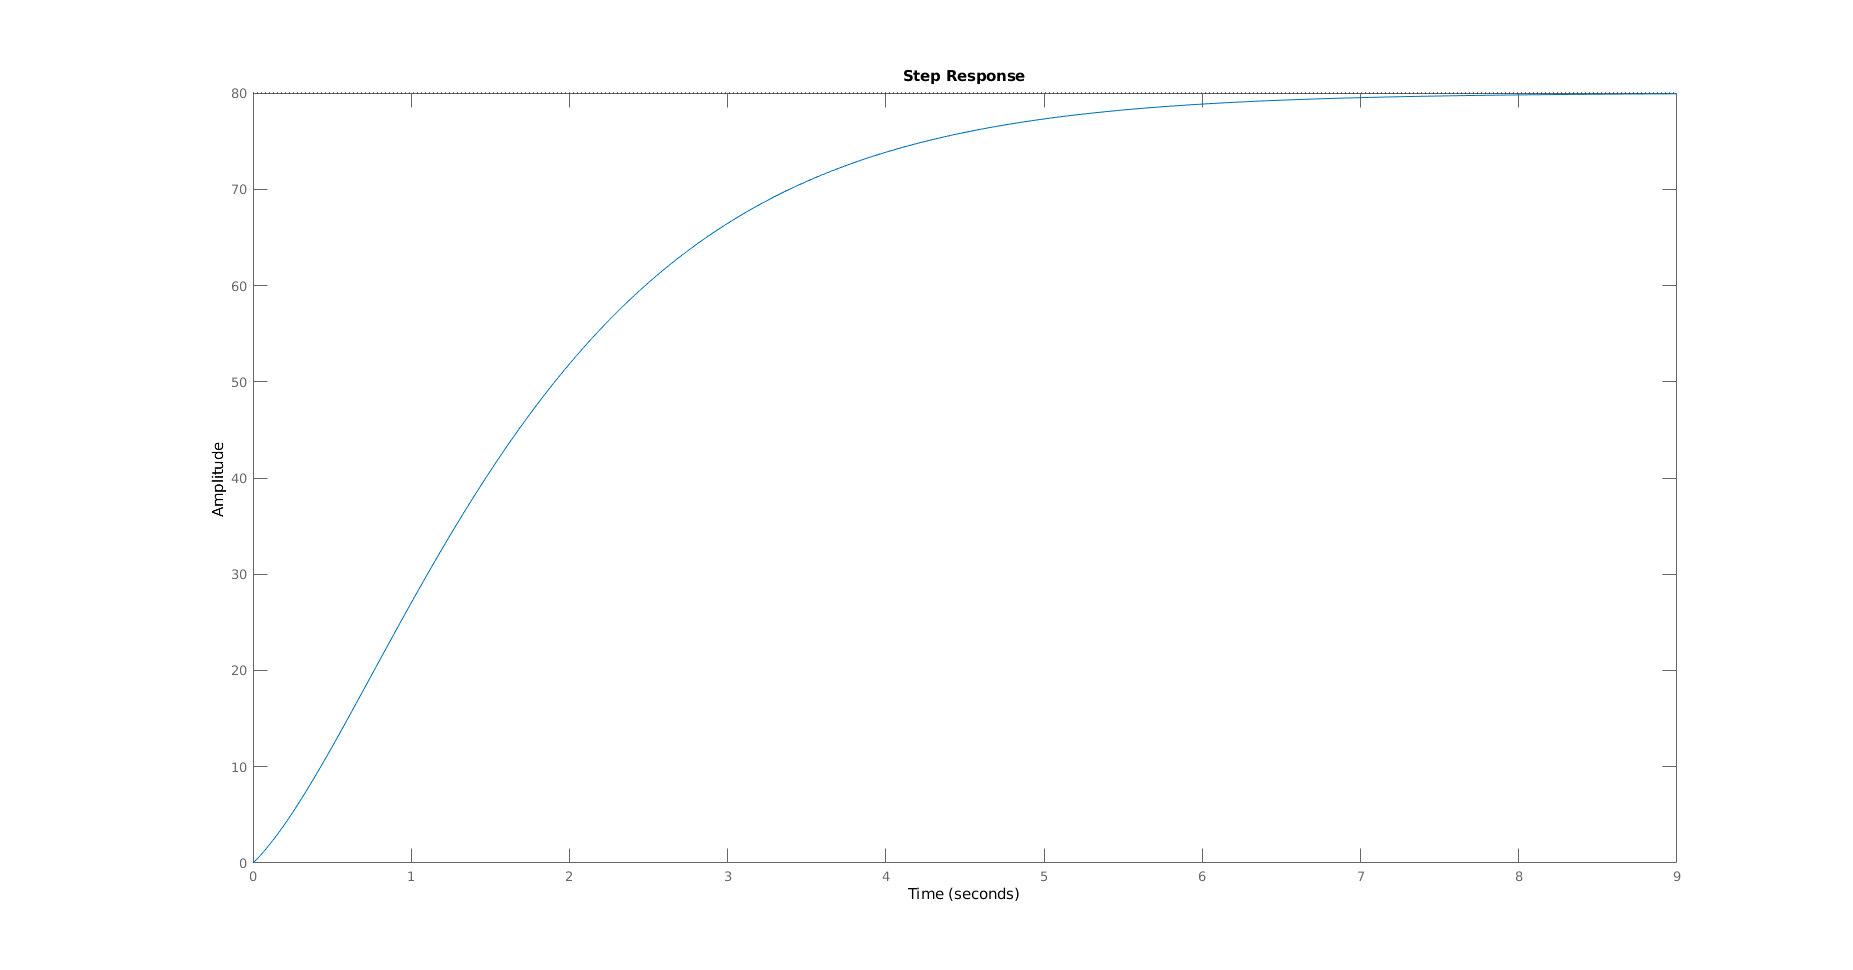
\includegraphics[width=\textwidth]{plot.png}
	\captionsetup{labelformat=empty}
	\caption{Abb. 2.2.1: Führungsübertragungsfuntion im Frequenzbereich}
\end{figure}

\end{document}
